\documentclass[12pt]{chmullighw}
\usepackage{tikz}
\usepackage{tikz-qtree}
\usepackage{algorithm2e}
\usetikzlibrary{shapes,chains,fit,shapes,matrix}
\usepackage{multicol}


% info for header block in upper right hand corner
\name{Chris Mulligan}
\uni{clm2186}
\class{COMS3137 Data Structures \& Algorithms}
\professor{Hershkop}
\assignment{Theory 5}
\duedate{November 21, 2013, \hspace{1em}  2 Days Late}

\lstset{language=Java, numbers=none, frame=l, captionpos=n}
\begin{document}
\problemlist{Theory 5} %Give us a nice big title
\begin{enumerate}

\item The initial table is: 

\begin{tabular}{ r | c | c | l }
Node & Distance & Parent & Visited \\
\hline
A & 0        &   &  \\
B & $\infty$ &   &  \\
C & $\infty$ &   &  \\
D & $\infty$ &   &  \\
E & $\infty$ &   &  \\
F & $\infty$ &   &  \\
G & $\infty$ &   &  \\
\end{tabular}


An intermediate table after exploring nodes A, C, B is: 

\begin{tabular}{ r | c | c | l }
Node & Distance & Parent & Visited \\
\hline
A & 0        &   &  \\
B & 5        & A & \checkmark \\
C & 3        & A & \checkmark \\
D & 10       & C &  \\
E & 8        & B &  \\
F & $\infty$ &   &  \\
G & 6        & B &  \\
\end{tabular}

The final table is: 

\begin{tabular}{ r | c | c | l }
Node & Distance & Parent & Visited \\
\hline
A & 0 &   & \checkmark \\
B & 5 & A & \checkmark \\
C & 3 & A & \checkmark \\
D & 9 & E & \checkmark \\
E & 7 & G & \checkmark \\
F & 8 & E & \checkmark \\
G & 6 & B & \checkmark \\
\end{tabular}

\newpage
\item Initial: \\
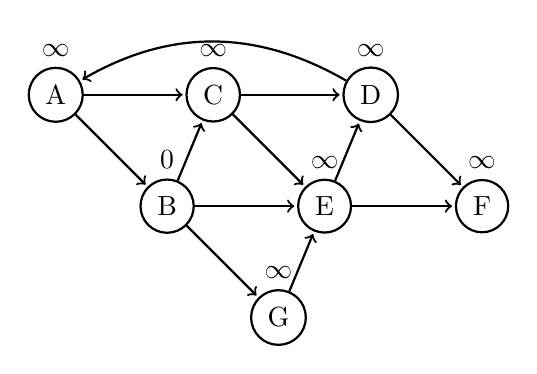
\begin{tikzpicture}[->,node distance=2cm, shorten >=1pt, thick]
\tikzstyle{nd}=[circle,draw=black,text=black]
\node[nd, label={$\infty$}] (A)                    {A};
\node[nd, label={0}]        (B) [below right of=A] {B};
\node[nd, label={$\infty$}] (C) [      right of=A] {C};
\node[nd, label={$\infty$}] (D) [      right of=C] {D};
\node[nd, label={$\infty$}] (E) [below right of=C] {E};
\node[nd, label={$\infty$}] (F) [below right of=D] {F};
\node[nd, label={$\infty$}] (G) [below right of=B] {G};
\path 
(A) edge              (C)
    edge              (B)
(B) edge              (G)
    edge              (C)
    edge              (E)
(G) edge              (E)
(C) edge              (E)
    edge              (D)
(E) edge              (D)
    edge              (F)
(D) edge              (F)
    edge [bend right] (A);
\end{tikzpicture}

Pop B, enqueue C, E, G. Current Queue: \texttt{[C,E,G]}: \\
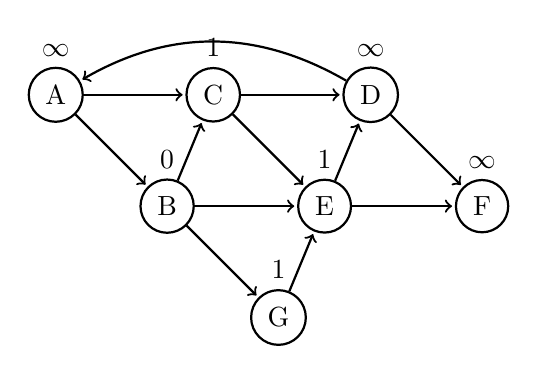
\begin{tikzpicture}[->,node distance=2cm, shorten >=1pt, thick]
\tikzstyle{nd}=[circle,draw=black,text=black]
\node[nd, label={$\infty$}] (A)                    {A};
\node[nd, label={0}]        (B) [below right of=A] {B};
\node[nd, label={1}] (C) [      right of=A] {C};
\node[nd, label={$\infty$}] (D) [      right of=C] {D};
\node[nd, label={1}] (E) [below right of=C] {E};
\node[nd, label={$\infty$}] (F) [below right of=D] {F};
\node[nd, label={1}] (G) [below right of=B] {G};
\path 
(A) edge              (C)
    edge              (B)
(B) edge              (G)
    edge              (C)
    edge              (E)
(G) edge              (E)
(C) edge              (E)
    edge              (D)
(E) edge              (D)
    edge              (F)
(D) edge              (F)
    edge [bend right] (A);
\end{tikzpicture}

Pop C, enqueue D, E. Current Queue: \texttt{[E,G,D,E]}: \\
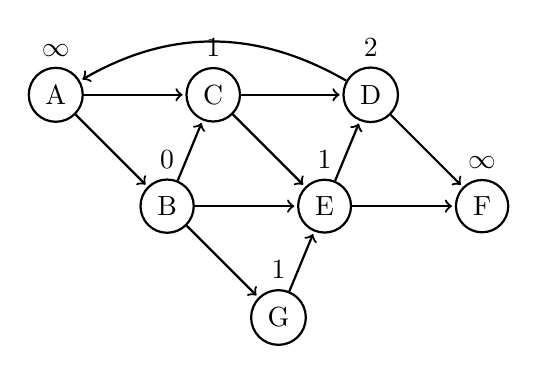
\begin{tikzpicture}[->,node distance=2cm, shorten >=1pt, thick]
\tikzstyle{nd}=[circle,draw=black,text=black]
\node[nd, label={$\infty$}] (A)                    {A};
\node[nd, label={0}]        (B) [below right of=A] {B};
\node[nd, label={1}]        (C) [      right of=A] {C};
\node[nd, label={2}]        (D) [      right of=C] {D};
\node[nd, label={1}]        (E) [below right of=C] {E};
\node[nd, label={$\infty$}] (F) [below right of=D] {F};
\node[nd, label={1}]        (G) [below right of=B] {G};
\path 
(A) edge              (C)
    edge              (B)
(B) edge              (G)
    edge              (C)
    edge              (E)
(G) edge              (E)
(C) edge              (E)
    edge              (D)
(E) edge              (D)
    edge              (F)
(D) edge              (F)
    edge [bend right] (A);
\end{tikzpicture}

Pop E, enqueue D, F. Current Queue: \texttt{[G,D,E,D,F]}: \\
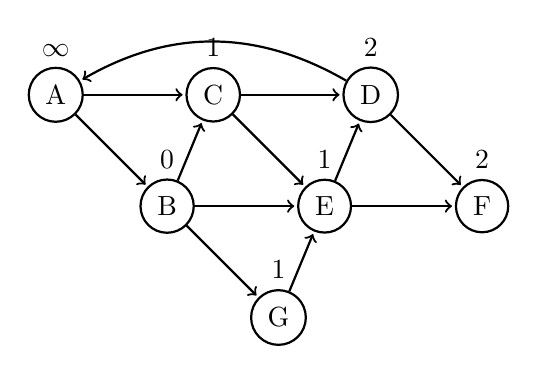
\begin{tikzpicture}[->,node distance=2cm, shorten >=1pt, thick]
\tikzstyle{nd}=[circle,draw=black,text=black]
\node[nd, label={$\infty$}] (A)                    {A};
\node[nd, label={0}]        (B) [below right of=A] {B};
\node[nd, label={1}]        (C) [      right of=A] {C};
\node[nd, label={2}]        (D) [      right of=C] {D};
\node[nd, label={1}]        (E) [below right of=C] {E};
\node[nd, label={2}]        (F) [below right of=D] {F};
\node[nd, label={1}]        (G) [below right of=B] {G};
\path 
(A) edge              (C)
    edge              (B)
(B) edge              (G)
    edge              (C)
    edge              (E)
(G) edge              (E)
(C) edge              (E)
    edge              (D)
(E) edge              (D)
    edge              (F)
(D) edge              (F)
    edge [bend right] (A);
\end{tikzpicture}

Pop G, enqueue E. Current Queue: \texttt{[D,E,D,F,E]}: \\
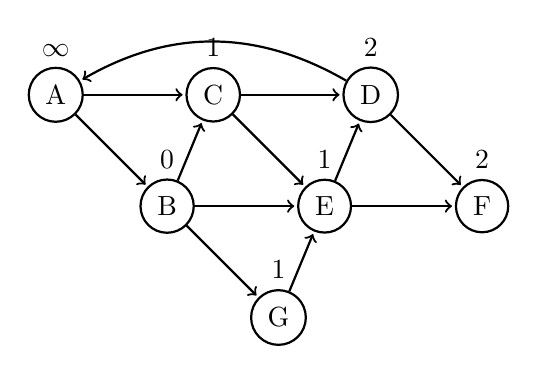
\begin{tikzpicture}[->,node distance=2cm, shorten >=1pt, thick]
\tikzstyle{nd}=[circle,draw=black,text=black]
\node[nd, label={$\infty$}] (A)                    {A};
\node[nd, label={0}]        (B) [below right of=A] {B};
\node[nd, label={1}]        (C) [      right of=A] {C};
\node[nd, label={2}]        (D) [      right of=C] {D};
\node[nd, label={1}]        (E) [below right of=C] {E};
\node[nd, label={2}]        (F) [below right of=D] {F};
\node[nd, label={1}]        (G) [below right of=B] {G};
\path 
(A) edge              (C)
    edge              (B)
(B) edge              (G)
    edge              (C)
    edge              (E)
(G) edge              (E)
(C) edge              (E)
    edge              (D)
(E) edge              (D)
    edge              (F)
(D) edge              (F)
    edge [bend right] (A);
\end{tikzpicture}

Pop D, enqueue A. Current Queue: \texttt{[E,D,F,E,A]}: \\
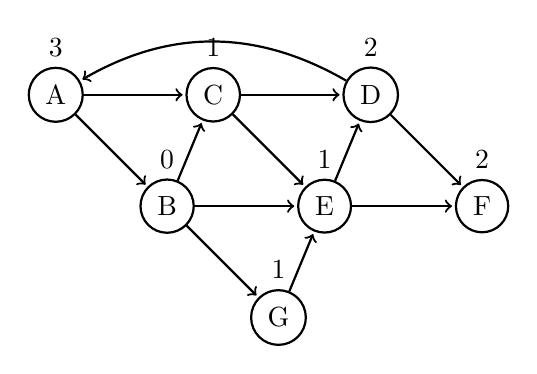
\begin{tikzpicture}[->,node distance=2cm, shorten >=1pt, thick]
\tikzstyle{nd}=[circle,draw=black,text=black]
\node[nd, label={3}]        (A)                    {A};
\node[nd, label={0}]        (B) [below right of=A] {B};
\node[nd, label={1}]        (C) [      right of=A] {C};
\node[nd, label={2}]        (D) [      right of=C] {D};
\node[nd, label={1}]        (E) [below right of=C] {E};
\node[nd, label={2}]        (F) [below right of=D] {F};
\node[nd, label={1}]        (G) [below right of=B] {G};
\path 
(A) edge              (C)
    edge              (B)
(B) edge              (G)
    edge              (C)
    edge              (E)
(G) edge              (E)
(C) edge              (E)
    edge              (D)
(E) edge              (D)
    edge              (F)
(D) edge              (F)
    edge [bend right] (A);
\end{tikzpicture}

Exhaust remaining queue, but no changes remain. Thus above is final results.

\begin{tabular}{ r | l }
Node & Distance \\
\hline
A & 3 \\
B & 0 \\
C & 1 \\
D & 2 \\
E & 1 \\
F & 2 \\
G & 1 \\
\end{tabular}

\item Given $n$ nodes, $m$ edges, and a graph represented as an adjacency table,
with a hash table to locate nodes in the array\ldots

insertVertex() will take \BigO{1}. We need to create a vertex at the end of the
array we're using to store nodes, which like most ArrayLists should be an
amortized constant operation (we only need to grow the array once it's currently
full).

deleteVertex() ends up taking \BigO{m}. Finding the vertex is \BigO{1}, it's
constant to remove it from the hash table, and then either \BigO{n} to
remove it from the array and compact the array, or just \BigO{1} if we
lazily delete.  However, we finally have to remove all edges pointing to this
vertex, so we need to do a \BigO{m} scan through all edges to delete them, but
fortunately each delete is constant. Thus the overall time is \BigO{n+m} and
assuming $m \approx kn$ this is \BigO{n}.

\item {\em Note: links above are left to right, links below are from right to left}

\begin{enumerate} \renewcommand{\labelenumii}{\alph{enumii}.}
    \item Arbitrary union

        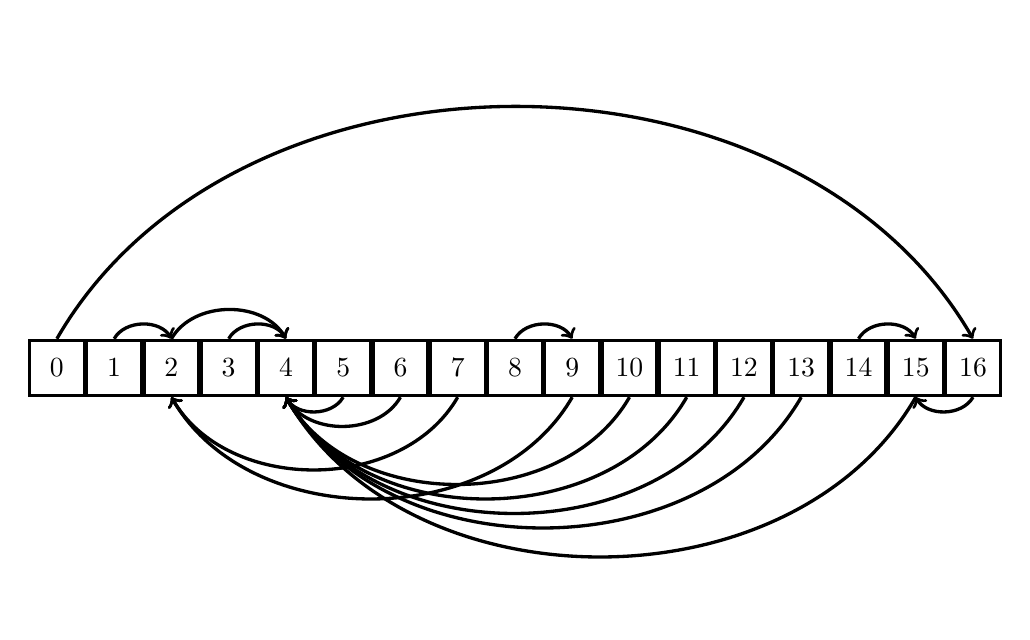
\begin{tikzpicture}
        \tikzstyle{every path}=[very thick]

        \edef\sizetape{.7cm}
        \tikzstyle{ht}=[draw,minimum size=\sizetape]
        \tikzstyle{num}=[draw=none]
        \tikzstyle{value}=[draw]

        \begin{scope}[start chain=1 going right,node distance=-0.15mm]
        \foreach \x in {0, 1,...,16} {
            \node [on chain=1,ht] (\x) {};
            \node [num] at (\x.center) (\x_label) {$\x$};
        };
        \end{scope}
        \draw[->, bend left=60]  (1.north) to  (2.north);  % 1->2
        \draw[->, bend left=60]  (3.north) to  (4.north);  % 3->4
        \draw[->, bend left=60]  (5.south) to  (4.south);  % 3->5
        \draw[->, bend left=60]  (7.south) to  (2.south);  % 1->7
        \draw[->, bend left=60]  (6.south) to  (4.south);  % 3->6
        \draw[->, bend left=60]  (8.north) to  (9.north);  % 8->9
        \draw[->, bend left=60]  (9.south) to  (2.south);  % 1->8
        \draw[->, bend left=60] (10.south) to  (4.south);  % 3->10
        \draw[->, bend left=60] (11.south) to  (4.south);  % 3->11
        \draw[->, bend left=60] (12.south) to  (4.south);  % 3->12
        \draw[->, bend left=60] (13.south) to  (4.south);  % 3->13
        \draw[->, bend left=60] (14.north) to (15.north);  % 14->15
        \draw[->, bend left=60]  (0.north) to (16.north);  % 16->0
        \draw[->, bend left=60] (16.south) to (15.south);  % 14->16
        \draw[->, bend left=60]  (2.north) to  (4.north);  % 1->3
        \draw[->, bend left=60] (15.south) to  (4.south);  % 1->14
        \end{tikzpicture}

\item union by height:

        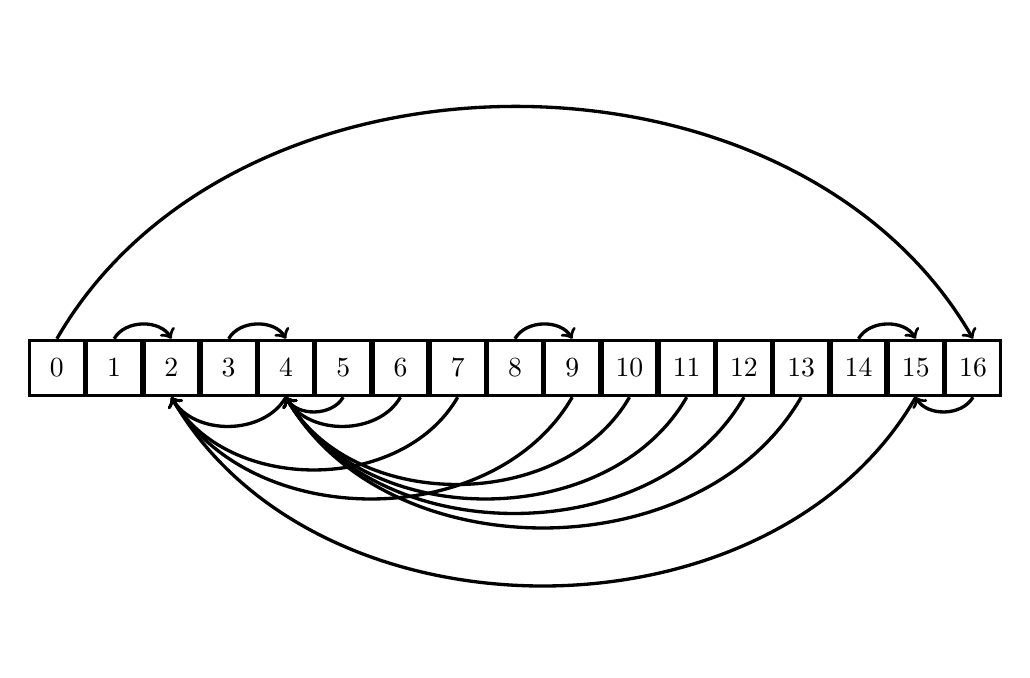
\begin{tikzpicture}
        \tikzstyle{every path}=[very thick]

        \edef\sizetape{.7cm}
        \tikzstyle{ht}=[draw,minimum size=\sizetape]
        \tikzstyle{num}=[draw=none]
        \tikzstyle{value}=[draw]

        \begin{scope}[start chain=1 going right,node distance=-0.15mm]
        \foreach \x in {0, 1,...,16} {
            \node [on chain=1,ht] (\x) {};
            \node [num] at (\x.center) (\x_label) {$\x$};
        };
        \end{scope}
        \draw[->, bend left=60]  (1.north) to  (2.north);  % 1->2
        \draw[->, bend left=60]  (3.north) to  (4.north);  % 3->4
        \draw[->, bend left=60]  (5.south) to  (4.south);  % 3->5
        \draw[->, bend left=60]  (7.south) to  (2.south);  % 1->7
        \draw[->, bend left=60]  (6.south) to  (4.south);  % 3->6
        \draw[->, bend left=60]  (8.north) to  (9.north);  % 8->9
        \draw[->, bend left=60]  (9.south) to  (2.south);  % 1->8
        \draw[->, bend left=60] (10.south) to  (4.south);  % 3->10
        \draw[->, bend left=60] (11.south) to  (4.south);  % 3->11
        \draw[->, bend left=60] (12.south) to  (4.south);  % 3->12
        \draw[->, bend left=60] (13.south) to  (4.south);  % 3->13
        \draw[->, bend left=60] (14.north) to (15.north);  % 14->15
        \draw[->, bend left=60]  (0.north) to (16.north);  % 16->0
        \draw[->, bend left=60] (16.south) to (15.south);  % 14->16
        \draw[->, bend left=60]  (4.south) to  (2.south);  % 1->3
        \draw[->, bend left=60] (15.south) to  (2.south);  % 1->14
        
        \end{tikzpicture}


    \item union by size:

        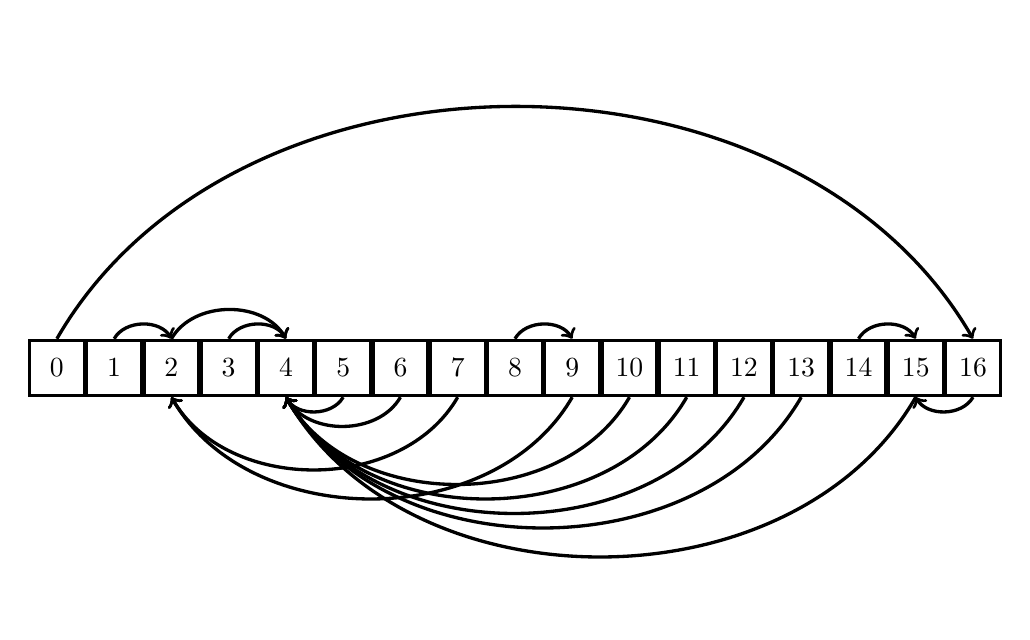
\begin{tikzpicture}
        \tikzstyle{every path}=[very thick]

        \edef\sizetape{.7cm}
        \tikzstyle{ht}=[draw,minimum size=\sizetape]
        \tikzstyle{num}=[draw=none]
        \tikzstyle{value}=[draw]

        \begin{scope}[start chain=1 going right,node distance=-0.15mm]
        \foreach \x in {0, 1,...,16} {
            \node [on chain=1,ht] (\x) {};
            \node [num] at (\x.center) (\x_label) {$\x$};
        };
        \end{scope}
        \draw[->, bend left=60]  (1.north) to  (2.north);  % 1->2
        \draw[->, bend left=60]  (3.north) to  (4.north);  % 3->4
        \draw[->, bend left=60]  (5.south) to  (4.south);  % 3->5
        \draw[->, bend left=60]  (7.south) to  (2.south);  % 1->7
        \draw[->, bend left=60]  (6.south) to  (4.south);  % 3->6
        \draw[->, bend left=60]  (8.north) to  (9.north);  % 8->9
        \draw[->, bend left=60]  (9.south) to  (2.south);  % 1->8
        \draw[->, bend left=60] (10.south) to  (4.south);  % 3->10
        \draw[->, bend left=60] (11.south) to  (4.south);  % 3->11
        \draw[->, bend left=60] (12.south) to  (4.south);  % 3->12
        \draw[->, bend left=60] (13.south) to  (4.south);  % 3->13
        \draw[->, bend left=60] (14.north) to (15.north);  % 14->15
        \draw[->, bend left=60]  (0.north) to (16.north);  % 16->0
        \draw[->, bend left=60] (16.south) to (15.south);  % 14->16
        \draw[->, bend left=60]  (2.north) to  (4.north);  % 1->3
        \draw[->, bend left=60] (15.south) to  (4.south);  % 1->14
        \end{tikzpicture}

\end{enumerate}

\item Quicksort and merge sort are both reasonable \BigO{n \log n} sorts
suitable for a range of problems. I would generally default to using quicksort,
since it's typically faster in real world problems on real world systems. The
key differences are that quicksort is generally unstable, and quicksort doesn't
work as well with non-array-like data structures. For example, merge sort is much
easier to implement for linked lists, because the append operation is cheap, but
random access is very expensive.

\newpage
\item
\begin{enumerate}
\item I have constructed an 8 vertex graph with 16 randomly generated edges (such that the graph is
connected and simple).

\begin{minipage}{0.65\linewidth}
\includegraphics[width=0.6\linewidth]{q6.png}
\end{minipage}
\begin{minipage}{0.2\linewidth}
Our edges are: \\
\begin{tabular}{l | l}
Weight & Edges \\
\hline
0 & 0 - 1 \\
1 & 3 - 1 \\
1 & 4 - 0 \\
2 & 1 - 7 \\
2 & 5 - 3 \\
2 & 6 - 3 \\
3 & 5 - 0 \\
5 & 2 - 3 \\
5 & 4 - 3 \\
6 & 2 - 6 \\
6 & 4 - 7 \\
7 & 4 - 1 \\
7 & 5 - 1 \\
7 & 6 - 0 \\
9 & 0 - 2 \\
9 & 7 - 5 \\
\end{tabular}
\end{minipage}

For Kruskal's Algorithm we process the sorted edges in order to add them to our
tree. Steps: Add 0-1; Add 3-1; Add 4-0; Add 1-7; Add 5-3; Add 6-3; skip 5-0; Add 2-3.

All nodes are now connected, and we've constructed our MST.

\begin{minipage}{0.7\linewidth}
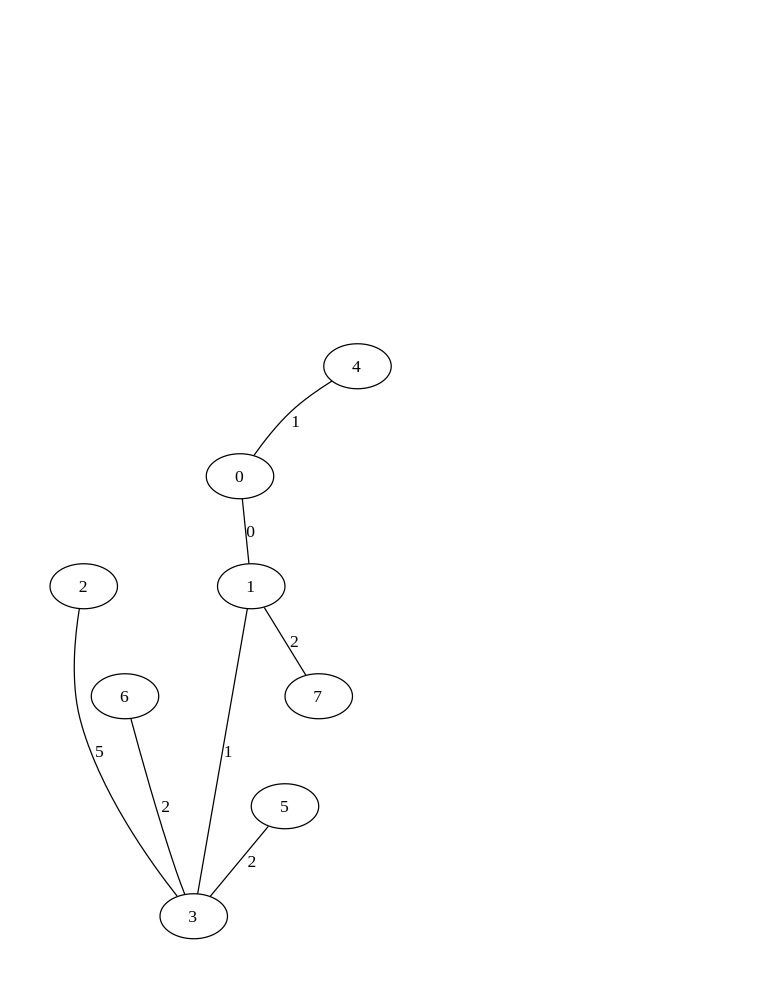
\includegraphics[width=0.35\linewidth]{q6_mst.png}
\end{minipage}
\begin{minipage}{0.2\linewidth}
Our edges are: \\
\begin{tabular}{l | l}
Weight & Edges \\
\hline
0 & 0 - 1 \\
1 & 3 - 1 \\
1 & 4 - 0 \\
2 & 1 - 7 \\
2 & 5 - 3 \\
2 & 6 - 3 \\
5 & 2 - 3 \\
\end{tabular}
\end{minipage}

\newpage

\item This problem is constructing a minimum spanning tree for the country. I
used a small python script, Josiah Carlson's disjoint set python library, and
Kruskal's algorithm. The least expensive 7 roads resulting in a connected graph are:
3---5, 1---8, 2---4, 2---8, 4---5, 6---7, 2---6.

\includegraphics[width=0.4\linewidth]{q6b.png}

\lstinputlisting[language=Python]{q6b.py}
\end{enumerate}

\item 
\begin{enumerate}
\item Drawn: \includegraphics[width=0.6\linewidth]{q7.png}

\item Assuming that given [2, 3, 4] we would push them on the stack in that order, thus we'd pop 4 off the stack first\ldots

DFS: 1, 4, 6, 7, 8, 5, 3, 2

\item BFS: 1, 2, 3, 4, 6, 5, 7, 8

\end{enumerate}

\end{enumerate} %end of questions
\end{document}
